\documentclass[a4paper,12pt]{article} % тип документа

%  Русский язык

\usepackage{wrapfig}
\usepackage[T2A]{fontenc}			% кодировка
\usepackage[utf8]{inputenc}			% кодировка исходного текста
\usepackage[english,russian]{babel}	% локализация и переносы

\usepackage{indentfirst} %Красная строка
\usepackage[a4paper,top=1.3cm,bottom=2cm,left=1.5cm,right=1.5cm,marginparwidth=0.75cm]{geometry}
\usepackage[usenames]{color}
\usepackage{colortbl}
\usepackage{float}

\usepackage{graphicx}%картинки
\usepackage{textcomp}%Номер
\usepackage{wrapfig}%обтекание текстом теблиц и картинок
%гиперссылки
\usepackage{hyperref}
\usepackage[rgb]{xcolor}
\hypersetup{     %гипперсылки
 colorlinks=true, %false:ссылки в рамках
 urlcolor=blue   %на URL
 }
% Заметки
\usepackage{todonotes}
% Номера формул(необязятельна, см. по ситуации)
%\mathtoolsset{showonlyrefs=true} % Показывать номера только у тех формул, на которые есть \eqref{} в тексте.

% Математика
\usepackage{amsmath,amsfonts,amssymb,amsthm,mathtools} 
\usepackage{wasysym}

\usepackage{euscript} % Шрифт Евклид
\usepackage{mathrsfs} % Красивый матшрифт

\begin{document}

\begin{titlepage}
\begin{center}
    {\large МОСКОВСКИЙ ФИЗИКО-ТЕХНИЧЕСКИЙ ИНСТИТУТ (НАЦИОНАЛЬНЫЙ ИССЛЕДОВАТЕЛЬСКИЙ УНИВЕРСИТЕТ)}
\end{center}
\begin{center}
    {\largeФизтех-школа аэрокосмических технологий}
\end{center}

\vspace{3.5cm}

\begin{center}
    
\includegraphics[width=0.4\linewidth]{hv_full.png}
\end{center}
\vspace{0.1cm}
{\huge
\begin{center}
    {\bf Лабораторная работа № 1}\\
    Эффективность алгоритмов сортировки    
\end{center}
}
\vspace{0.5cm}
\begin{flushright}
{\LARGE Автор:\\ 
Леонид Ефремов \\ 
\vspace{0.2cm}
Б03-403}
\end{flushright}
\vspace{3.5cm}
\begin{center}
    Долгопрудный 2024
\end{center}
\end{titlepage}

\tableofcontents
\section{Введение}

В данной лабораторной работе рассматриваются основные алгоритмы сортировки, их временная сложность и эффективность в зависимости от различных факторов, таких как размер входных данных и их первоначальная упорядоченность. Основное внимание уделяется анализу следующих алгоритмов: сортировка пузырьком, сортировка выбором, сортировка вставками, быстрая сортировка, сортировка кучей и сортировка слиянием.\par
Целью лабораторной работы является не только понимание теоретических аспектов временной сложности, но и приобретение практических навыков в реализации и тестировании алгоритмов сортировки. Результаты работы помогут лучше осознать, как выбор алгоритма может влиять на эффективность обработки данных в реальных приложениях.
\subsection{Эксперимент}
Для проведения эксперимента использовался компьютер на базе процессора "Ryzen 5 3600" в однопоточном режиме с фиксацией тактовой частоты на 3.6 ГГц при постоянном температурном режиме, двухканальная память ddr4 с фиксированной частотой на 2.4 ГГц. Замер времени производится через каждые 100 добавленных элементов. Управляющий код в приложении.
\section{Алгоритмы асимптротики $O(n^2)$}
\subsection{Демонстрация}
Для начала рассмотрим алгоритмы, простые в написании.\par
\begin{figure}[H]
    \centering
    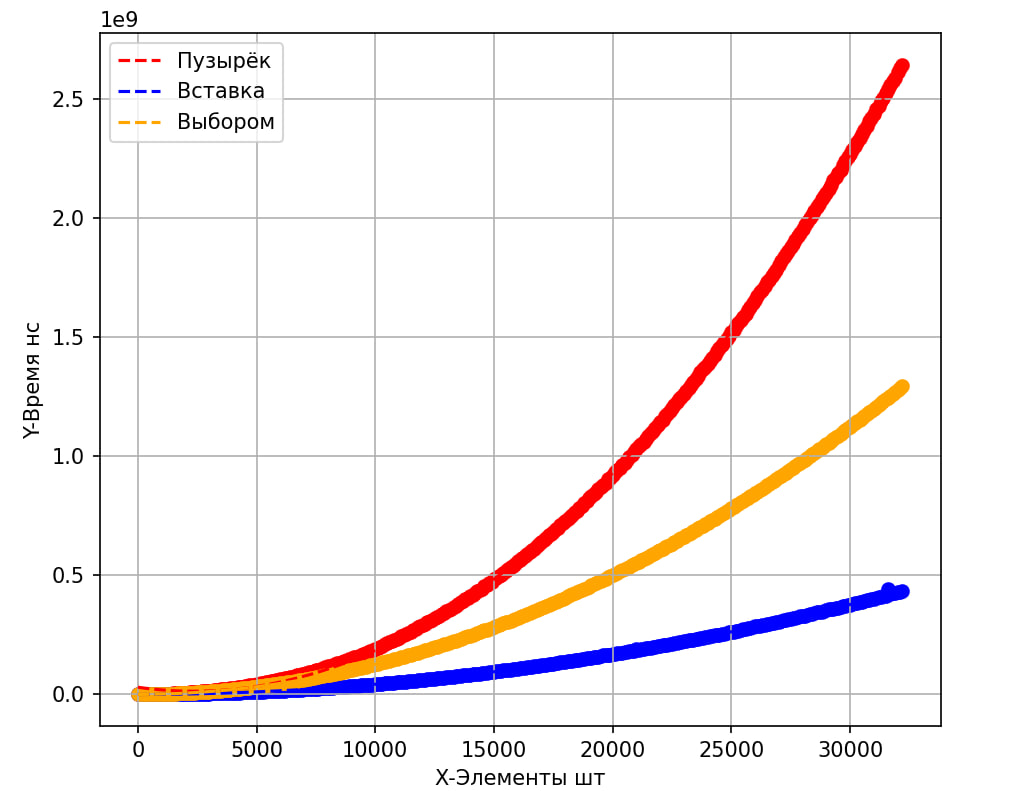
\includegraphics[width=0.7\textwidth]{img/first/O2.jpg}
    \caption{Сложность $O(n^2)$}
\end{figure} 
Для доказательства такой сложности используем логарифмический масштаб:
$ln(t)=ln(C)+2lnN$
\begin{figure}[!h]
    \centering
    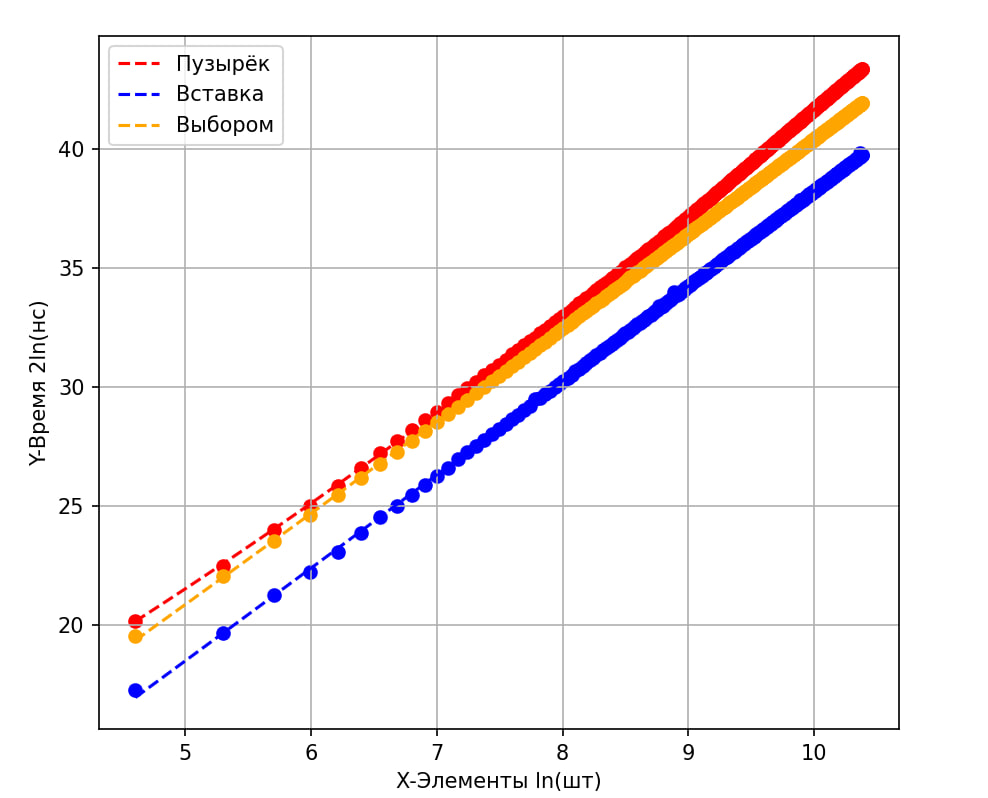
\includegraphics[width=0.7\textwidth]{img/first/O2ln.jpg}
    \caption{Доказательство сложности $O(n^2)$}
\end{figure} 
Имеем линейный вид графиков, квадратичная зависимость подтверждена.

\subsection{Сравнение оптимизаций}
\begin{figure}[H]
    \centering
    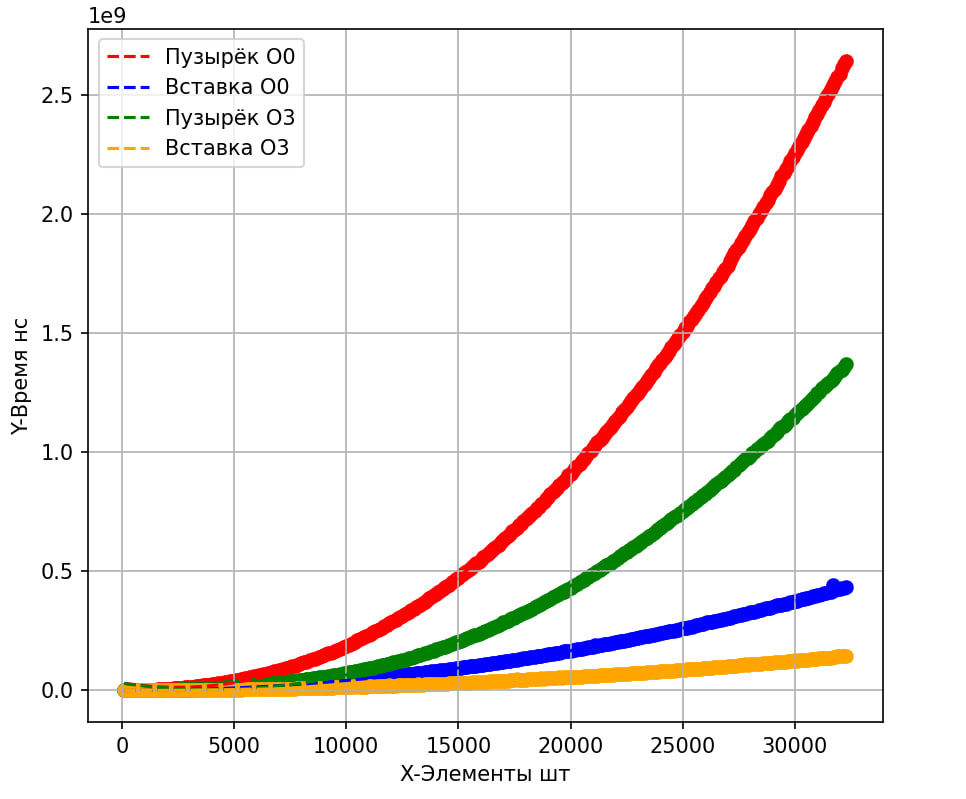
\includegraphics[width=0.7\textwidth]{img/first/optimO2.jpg}
    \caption{Демонстрация эффективности оптимизации для квадратичных алгоритмов}
\end{figure} 
\section{Алгоритмы асимптротики $O(NlogN)$}
\subsection{Демонстрация}
Сравним эффективные алгоритмы сортировки между собой.
\begin{figure}[H]
    \centering
    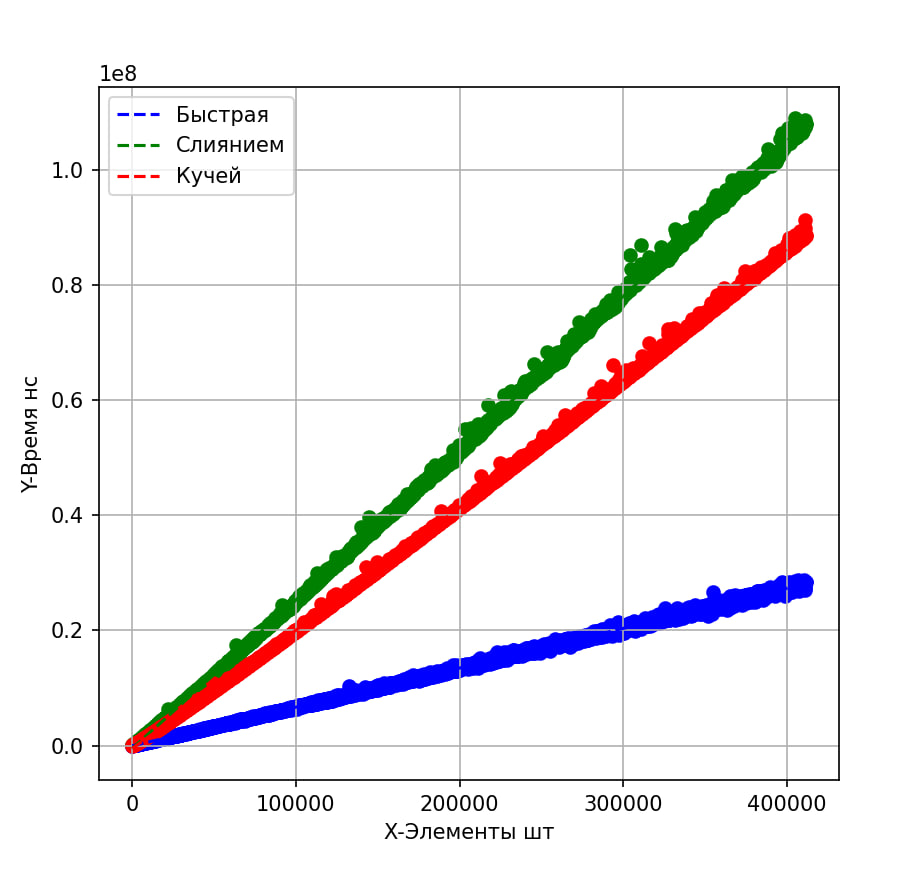
\includegraphics[width=0.55\textwidth]{img/first/qw.jpg}
    \caption{Сложность $O(NlogN)$}
\end{figure} 
Для доказательства такой сложности используем логарифмический масштаб:
$t=t/NlnN$
\begin{figure}[H]
    \centering
    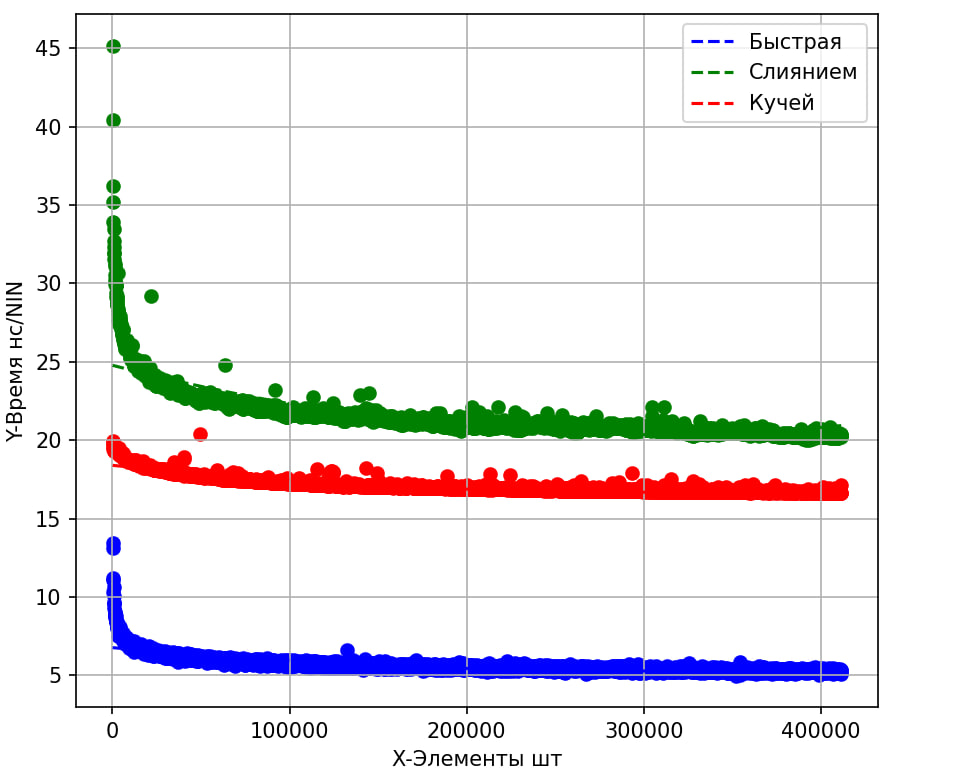
\includegraphics[width=0.7\textwidth]{img/first/qvln.jpg}
    \caption{Доказательство сложности $O(NlogN)$}
\end{figure} 
Имеем линейный вид графиков, логарифмическая зависимость подтверждена.

\subsection{Сравнение оптимизаций}
\begin{figure}[!h]
    \centering
    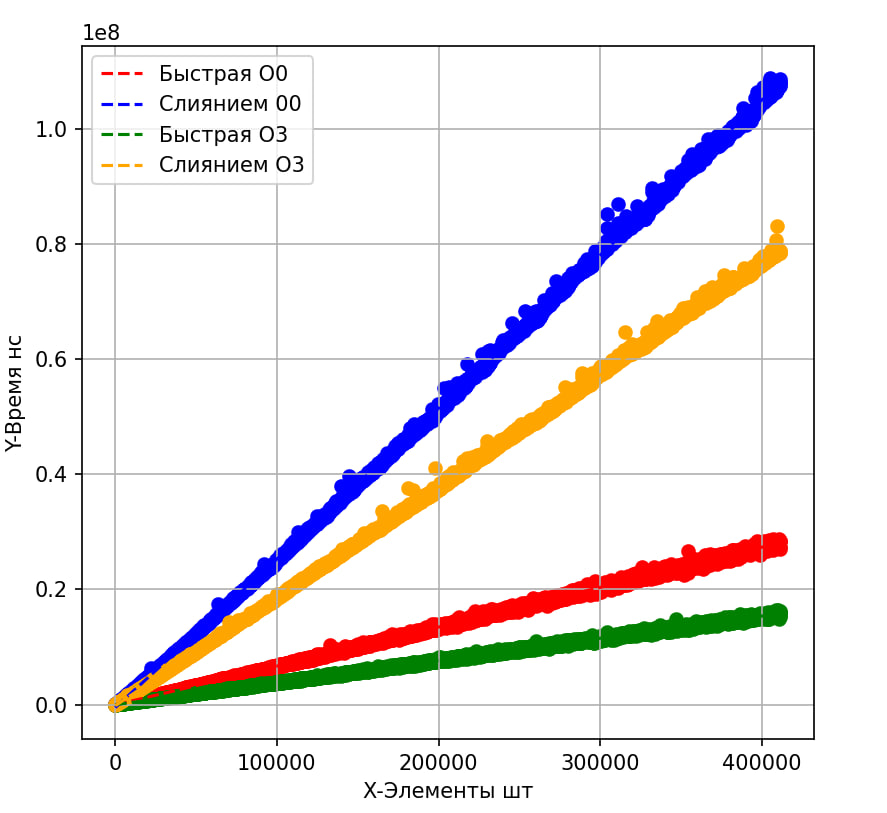
\includegraphics[width=0.5\textwidth]{img/first/qwoptim.jpg}
    \caption{Демонстрация эффективности оптимизации для логарифмических алгоритмов}
\end{figure} 
Быстрая сортировка оправдывает своё имя, даже её неоптимизированная версия превосходит конкурентов.

\section{$O(NlogN)$ и $O(N^2)$}
Для наглядности сравним алгоритмы сортировки разных рангов. Для более объективной картины, отключим оптимизации:
\begin{figure}[H]
    \centering
    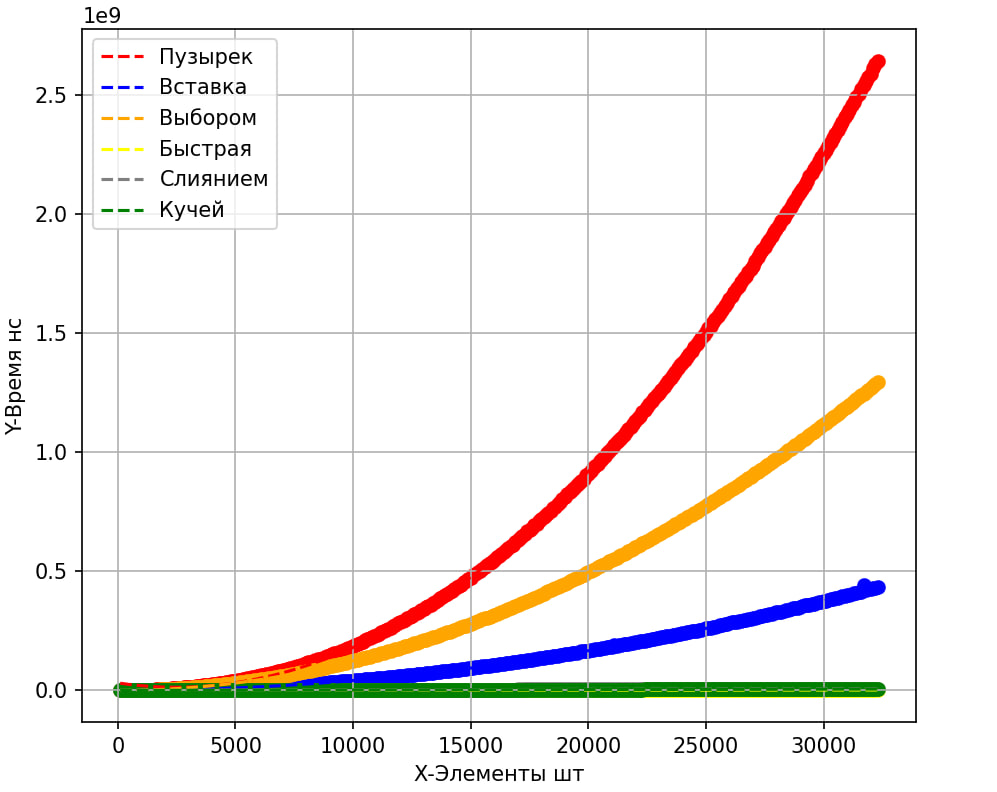
\includegraphics[width=0.7\textwidth]{img/first/all.jpg}
    \caption{Все алгоритмы сортировки}
\end{figure} 
\section{Зависимость от начальных данных}
Используем случайный, возрастающий и убывающий массив чисел:
\begin{figure}[H]
    \centering
    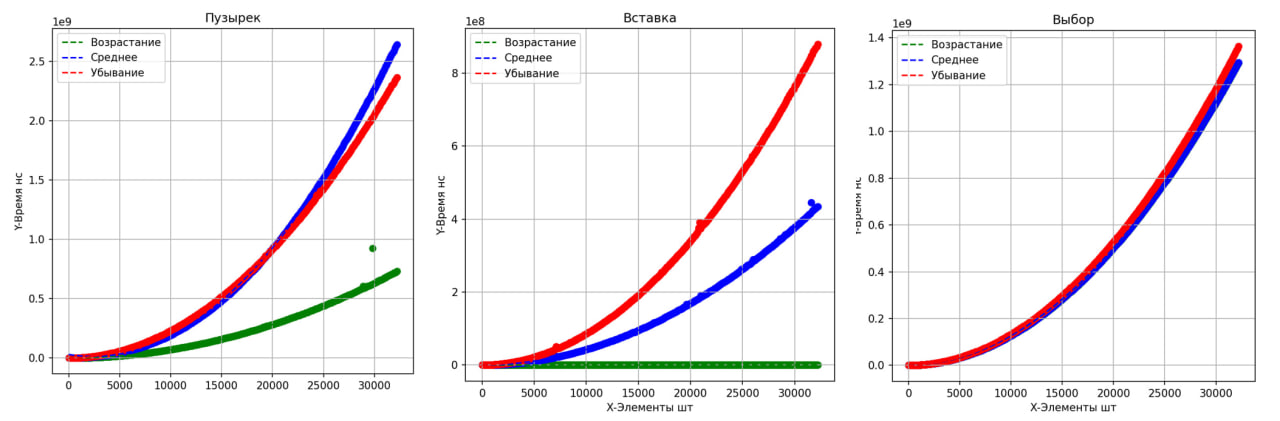
\includegraphics[width=0.99\textwidth]{tr1.jpg}
\end{figure} 
\begin{figure}[H]
    \centering
    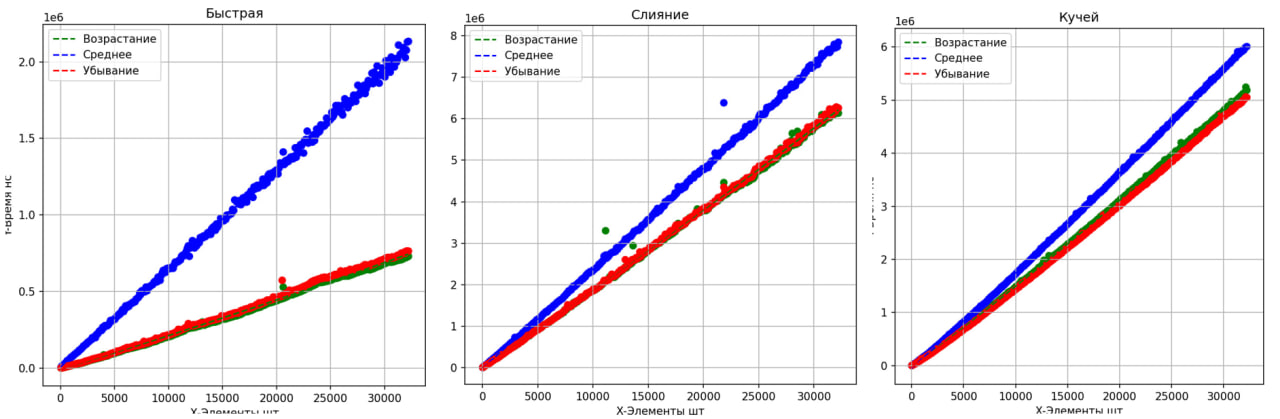
\includegraphics[width=0.99\textwidth]{tr2.jpg}
\end{figure} 
\section{C++ VS C\#}
Так как Python очевидно медленнее C++, сравним отца и его блудного объектно-ориентированного сына. Здесь уже схватка насмерть - максимальная оптимизация на обоих языках:
\begin{figure}[H]
    \centering
    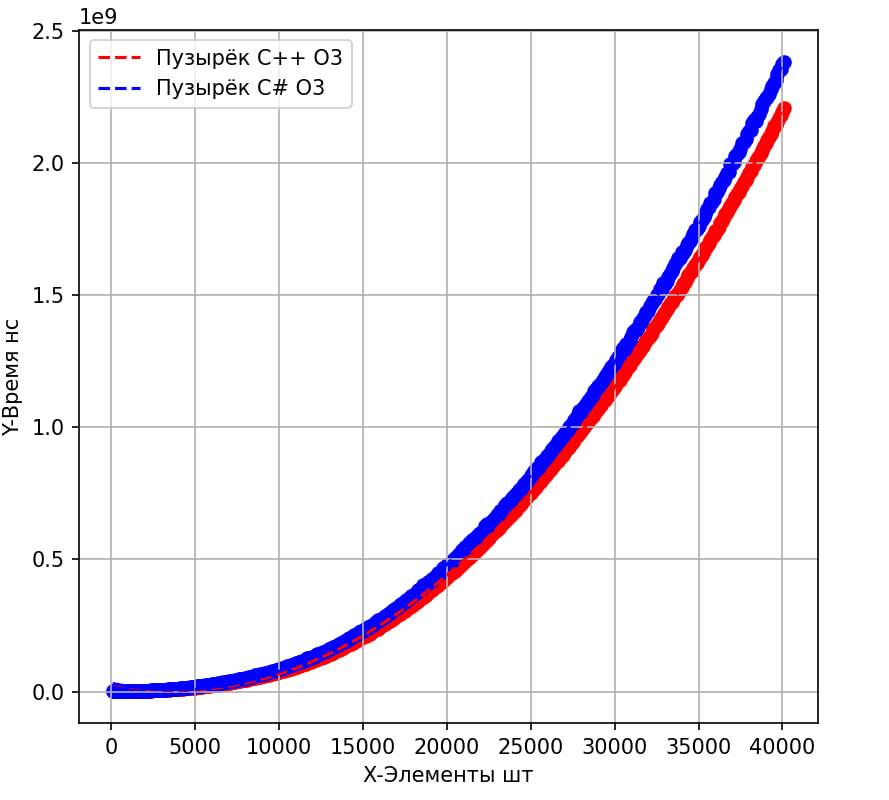
\includegraphics[width=0.7\textwidth]{img/last/compsl.jpg}
\end{figure} 
В первом раунде разница в производительности по времени неочевидна, однако C\# убивает C++, если речь заходит о удобстве написания кода и количестве подводных камней. Устроим бой на более совершенных алгоритмах:
\begin{figure}[H]
    \centering
    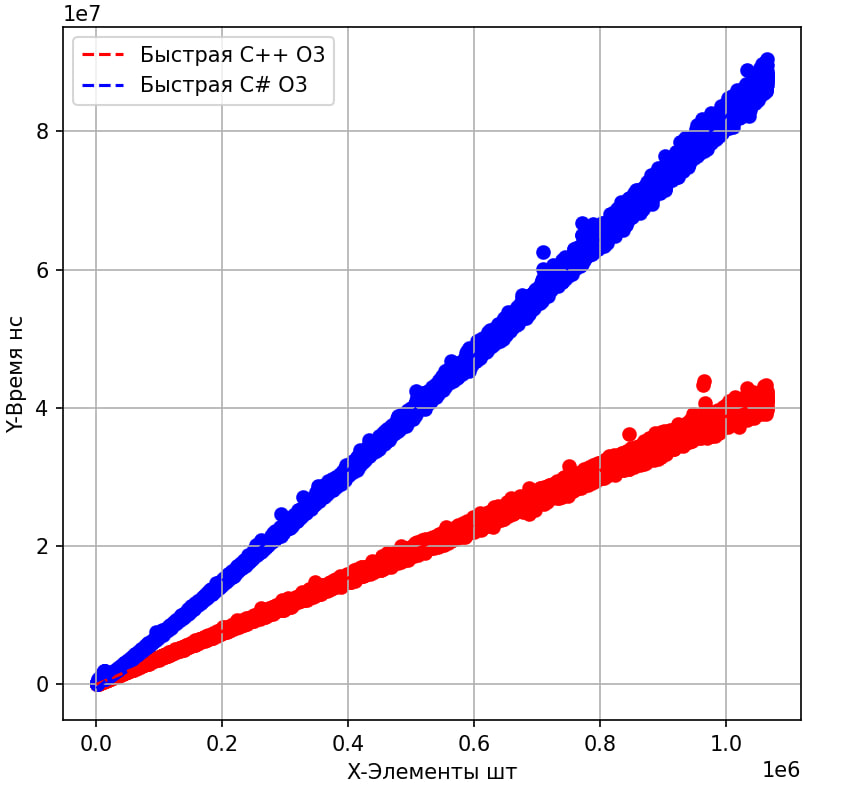
\includegraphics[width=0.7\textwidth]{img/last/compqw.jpg}
\end{figure} 
В быстрых алгоритмах ситуация печальнее: С++ значительно выигрывает.
\section{Сравнение мощности на малых массивах}
\begin{figure}[H]
    \centering
    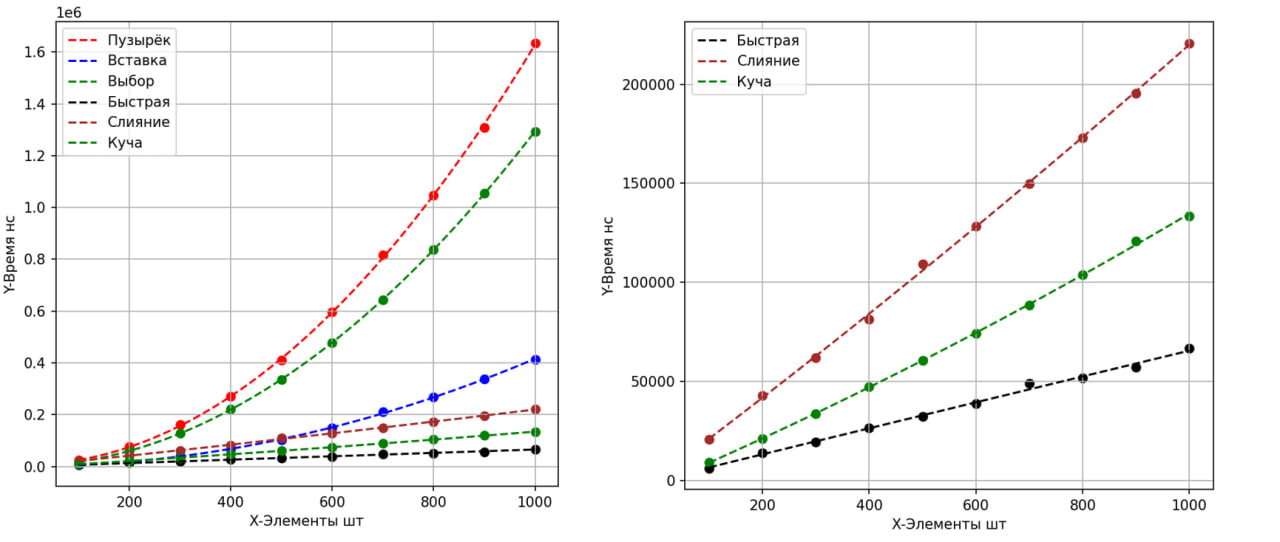
\includegraphics[width=0.99\textwidth]{p2.jpg}
\end{figure} 
Благодаря грамотной конфигукации эксперимента, всякие артефакты при замере времени отсутствуют даже при малых массивах. Быстрая сортировка - фаворит даже при малых массивах. Квадратичная сортировка вставкой эффективнее логарифмической сортировки слиянием при входных массивах длиной меньше 500 элементов.
\section{Вывод}
В ходе выполнения лабораторной работы была проведена сравнительная оценка временной эффективности различных алгоритмов сортировки, таких как пузырьковая сортировка, сортировка вставками, сортировка выбором, быстрая сортировка, сортировка кучей и сортировка слиянием. \par

Мы проанализировали время выполнения каждого алгоритма на различных наборах данных, включая уже отсортированные, случайные и обратные последовательности. Результаты эксперимента показали, что временная сложность алгоритмов существенно зависит от структуры входных данных.\par

1. Пузырьковая сортировка и сортировка выбором продемонстрировали наименьшую эффективность, особенно на больших объемах данных, с временной сложностью $O(n^2)$. Эти алгоритмы не рекомендуются для использования в реальных задачах, требующих быстрой обработки.\par

2. Быстрая сортировка, сортировка кучей и сортировка слиянием оказались наиболее эффективными для больших массивов, с временной сложностью $O(NlogN)$ в среднем случае. Быстрая сортировка оказалась быстрее во всех тестах.
В реальных приложениях предпочтение следует отдавать более эффективным алгоритмам, таким как быстрая сортировка или сортировка слиянием, особенно при работе с большими объемами данных.\par 

Полученные результаты подчеркивают важность анализа временной эффективности алгоритмов и выбора языка программирования при разработке программного обеспечения и оптимизации вычислительных процессов.
\end{document}